\section{Determination of yields from fit to $m_{jj}$ distribution in data sidebands}
\label{sec:yieldsDetermination}
% ---- ---- ---- ---- ---- ---- ---- ---- ---- ---- ---- ---- ---- ---- ---- ---- ---- ---- ---- ---- ---- ---- ----


\label{sec:mjj_fit}
In order to set limit on Higgs production cross section, we first need to 
estimate the total yields of various background components present in the 
data.
We extract the background yields from 
an unbinned maximum likelihood fit to the 
dijet invariant mass distribution $m_{jj}$,  
excluding the signal region (
$65~{\mbox{GeV}} < m_{jj} < 95~{\mbox{GeV}}$). 
Events in the signal region are later used 
to set Higgs exclusion limits. 
Table~\ref{tab:mjj_shapes_and_normalization} shows how the 
shape of each component is determined, and what constraints 
are applied to fit for the normalization. 
The main sources of 
systematics error are the uncertainties in the factorization 
and renormalization scales ($q^2$) and the matrix element -- parton shower 
matching scale in the the leading-order $W+$jets Monte Carlo, as well as 
the jet energy scale (JES) uncertainty. 
The results of the fit for 2-jet and 3-jet samples are shown 
in Fig.~\ref{fig:mjj_2jet} and Fig.~\ref{fig:mjj_3jet}, respectively. 
A clear peak from the Standard Model electroweak diboson 
$WW/WZ$ production can be seen in both plots. 
The resolution and yield for the diboson events are 
consistent with the Standard Model predictions computed up to 
the next-to-leading order in perturbation theory.
We extract the number of events in the signal mass window 
($65~{\mbox{GeV}} < m_{jj} < 95~{\mbox{GeV}}$) for each 
background process 
and plot their 4-body invariant mass distribution $m_{\ell\nu jj}$, 
as described in the next section.
%%%%%%%%%%%%%%%
\begin{table}[!ht]
  \begin{center}
 \caption{Determination of the $m_{jj}$ shape and normalization.}  
 \label{tab:mjj_shapes_and_normalization} 
 \begin{tabular} {l  c  c c c }
   \hline \hline
   Process                &    Shape                         &  Shape syst.           & Normalization   &  Norm. syst.\\  \hline
   $W+$jets               &    MC/ data                      &  $q^2$, matching, JES  & Unconstrained   &  Unconstrained \\
   diboson                &    MC                            &  JES                   & Constrain: CMS WW,WZ        &  Gaus $\sigma =15\%$ \\ 
   $t\bar{t}$, single top &    MC                            &  JES                   & Constrain: NLO        &  Gaus $\sigma =10\%$  \\ 
   $Z$+jets               &    MC                            &  JES                   & Constrain: NLO        &  Gaus $\sigma =15\%$  \\
   QCD                    &    data                          &  JES                   & Constrain: $m_T$ fit in data  &  Gaus $\sigma =50\%$  \\\hline \hline
 \end{tabular}
\end{center}
\end{table}
%%%%%%%%%%%%%%%%%%%%%%%%%%%%%%
%%%%%%%%%%%%%%%%%%%%
%%%%%%%%%%%%%%%%%%%%
\begin{figure}[h!t]
  {\centering
    \includegraphics[width=0.49\textwidth]{plots/kalanand_2jetsample/mJJ_Stacked.pdf}
    \includegraphics[width=0.49\textwidth]{plots/kalanand_2jetsample/mJJ-combined-fit-logY-truncated.pdf}
    \includegraphics[width=0.49\textwidth]{plots/kalanand_2jetsample/mJJ-combined-fit-subtracted-truncated.pdf}
    \includegraphics[width=0.49\textwidth]{plots/kalanand_2jetsample/mJJ-combined-fit-residual-truncated.pdf}

    \caption{Distribution of the dijet invariant mass for the 2-jet events in data and Monte Carlo: 
      (upper left) All background components stacked together, 
      (upper right) unstacked, (lower left) [Data -  All backgrounds except diboson],  
      (lower right) normalized residual between data and MC.}
    \label{fig:mjj_2jet}}
\end{figure}
%%%%%%%%%%%%%%%%%%%%
%%%%%%%%%%%%%%%%%%%%
\begin{figure}[h!t]
  {\centering
    \includegraphics[width=0.49\textwidth]{plots/kalanand_3jetsample/mJJ_Stacked.pdf}
    \includegraphics[width=0.49\textwidth]{plots/kalanand_3jetsample/mJJ-combined-fit-logY-truncated.pdf}
    \includegraphics[width=0.49\textwidth]{plots/kalanand_3jetsample/mJJ-combined-fit-subtracted-truncated.pdf}
    \includegraphics[width=0.49\textwidth]{plots/kalanand_3jetsample/mJJ-combined-fit-residual-truncated.pdf}

    \caption{Distribution of the dijet invariant mass for the 3-jet events in data and Monte Carlo: 
      (upper left) All background components stacked together, 
      (upper right) unstacked, (lower left) [Data -  All backgrounds except diboson],  
      (lower right) normalized residual between data and MC.}
    \label{fig:mjj_3jet}}
\end{figure}
